\subsection{Objekterkennung}
\label{sec_objDet}
Die Objekterkennung basiert auf einem ähnlichen Verfahren wie das vorgestellte CSurvey Projekt\cite{Albiez2015CSurveyA}.\\
Da ein Farberkennung aufgrund der Sichtbedingungen nicht in Frage kommt wird im ersten Schritt das RGB-Bild in ein Graustufenbild umgewandelt. In diesem Bild sollte ein gesuchtes Objekt einen höheren Helligkeitswert besitzen, als der Meeresboden (siehe \ref{brightCurve_real} und \ref{brightCurve_sim}).\\
Aus Erfahrungswerten früherer Projekte riet Christopher Gaudig mir, die Rotwerte der Bilder zu betrachten, da oftmals der Meeresboden und trübes Wasser geringe Rotwerte haben. In den Abbildungen \ref{redCurve_real} und \ref{redCurve_sim} ist dies zu beobachten. Die Kurven sehen denen der Helligkeitswerte sehr ähnlich, jedoch sind die Ausschläge des Objektes in den Rotwerten höher. Die hat zur Folge, dass der Templatewert ebenso höher ist und das Objekt besser erkannt werden kann.\\
Im nächsten Schritt wird mithilfe eines Templates ein Binärbild erzeugt. Das Template zeichnet sich durch drei Pixelangaben aus. Die \textit{Testpixel} geben einen Bereich an, der im aktuellen Schritt geprüft wird. Die \textit{Checkpixel} geben den Bereich rechts und links neben dem Testbereich an und bilden den Referenzwert. Die \textit{Borderpixel} geben einen Bereich zwischen Test- und Checkbereich an, der ignoriert wird. Ein solches Template wird auf jeden Pixel im Bild angewendet um zu entscheiden, ob der betrachte Pixel Teil des Objektes sein kann. Dies ist der Fall, wenn der Wert eines Pixels [\ref{templateValue}] einen Schwellwert übersteigt.\\
Die verschiedenen Bereiche lassen sich in drei Mengen an Indizes definieren.
\begin{ownequation}[H]
\begin{eqnarray}
TP_i = \{i-\frac{\#TP}{2} \dots i \dots i+\frac{\#TP}{2}\}\\
LC_i = \{i-\frac{\#TP}{2}-\#BP-\#CP \dots i-\frac{\#TP}{2}-\#BP\}\\
RC_i = \{i-i+\frac{\#TP}{2}+\#BP \dots \frac{\#TP}{2}+\#BP+\#CP\}\\
\end{eqnarray}
\caption{Testbereich ($TP$) und Checkbereiche ($LC$ und $RC$) für ein Pixel mit Index $i$}
\end{ownequation}
Mit diesen Mengen lässt sich dann die Berechnung eines Templatewerten ($TV$) zu definieren.
\begin{ownequation}[H]
\begin{eqnarray}
TV_i = \frac{\sum_{x \in TP_i} image(x))}{\#TP} - \left(\frac{\sum_{y_1 \in LC_i} image(y_1) + \sum_{y_2 \in RC_i} image(y_2)}{2 \cdot \#CP}\right)
\end{eqnarray}
%\begin{split}
%&((\sum_{y_1 = i-TP/2-BP-CP:i-TP/2-BP} image(y_1)):CP +\\
%&(\sum_{y_2 = i+TP/2+BP:i+TP/2+BP+CP} image(y_2)):CP)
%\end{split}
%\end{equation}
\caption{Templatewertberechnung für ein Pixel $i$}
\label{templateValue}
\end{ownequation}


\begin{figure}[H]
\begin{tabular}{cc}
\multicolumn{2}{c}{\subfloat[Originalbild]{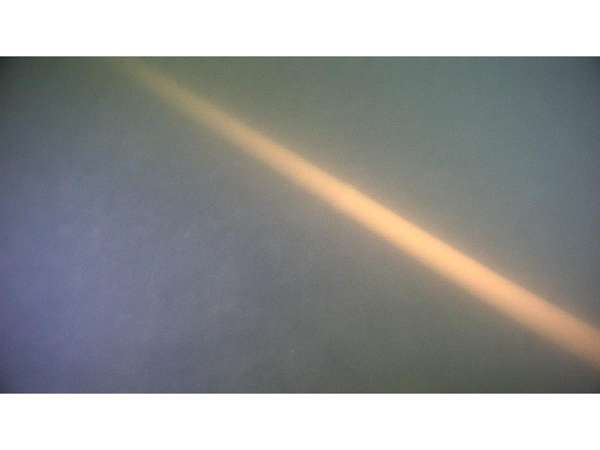
\includegraphics[height=0.33\textheight,width=0.5\textwidth]{imageProcessing/realPipe/004orgImstart.jpg}}}\\
%\subfloat[Originalbild]{\includegraphics[height=0.33\textheight,width=0.5\textwidth]{imageProcessing/3orgImFin.jpg}}\\
\subfloat[Helligkeitsverlauf einer Bildzeile im oberen Drittel des Bildes]{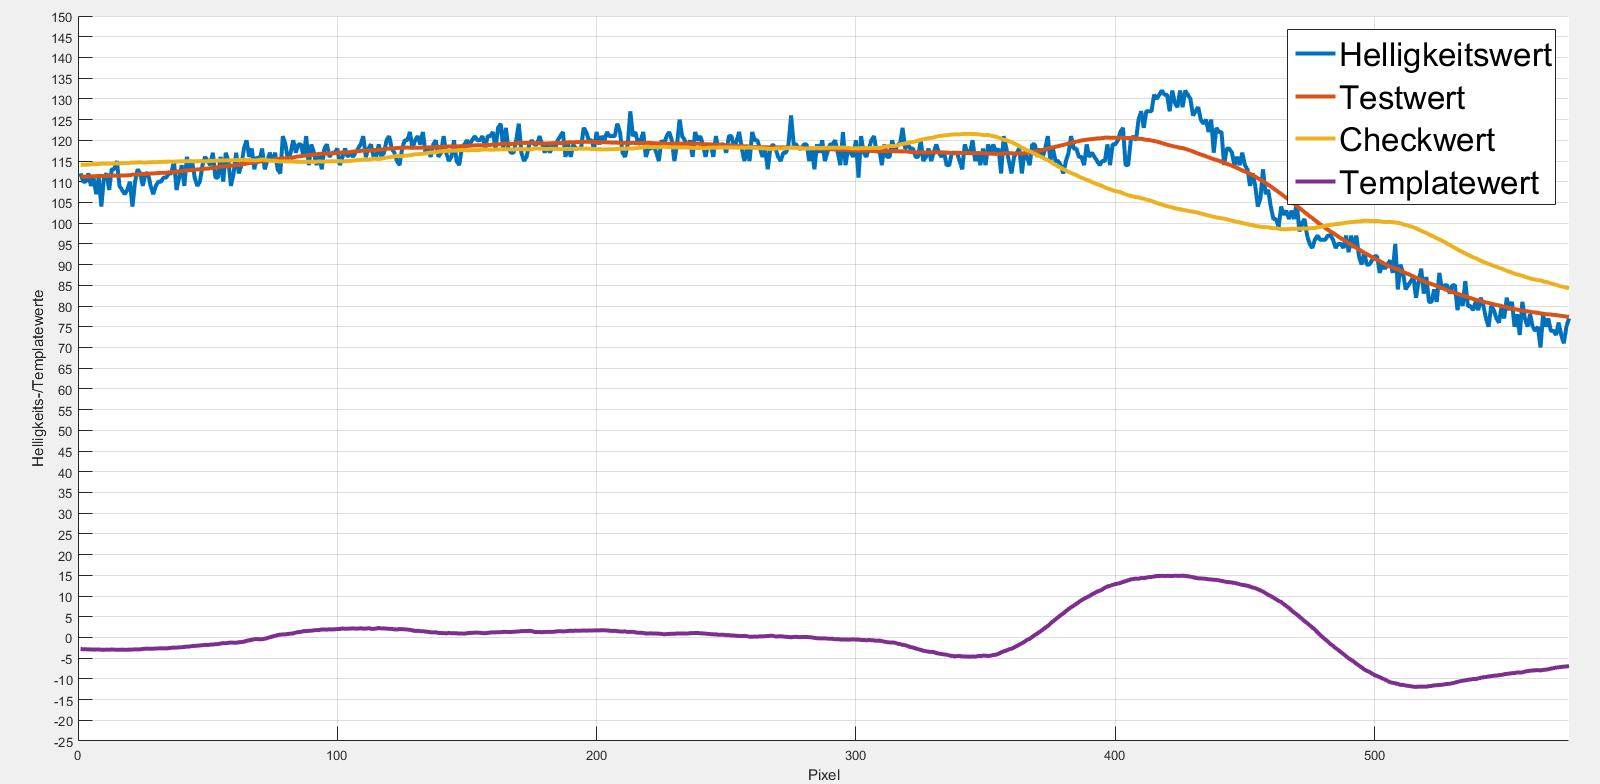
\includegraphics[height=0.33\textheight,width=0.5\textwidth]{1hellRealGut.jpg}\label{brightCurve_real}}&
\subfloat[Rotwertverlauf einer Bildzeile im oberen Drittel des Bildes]{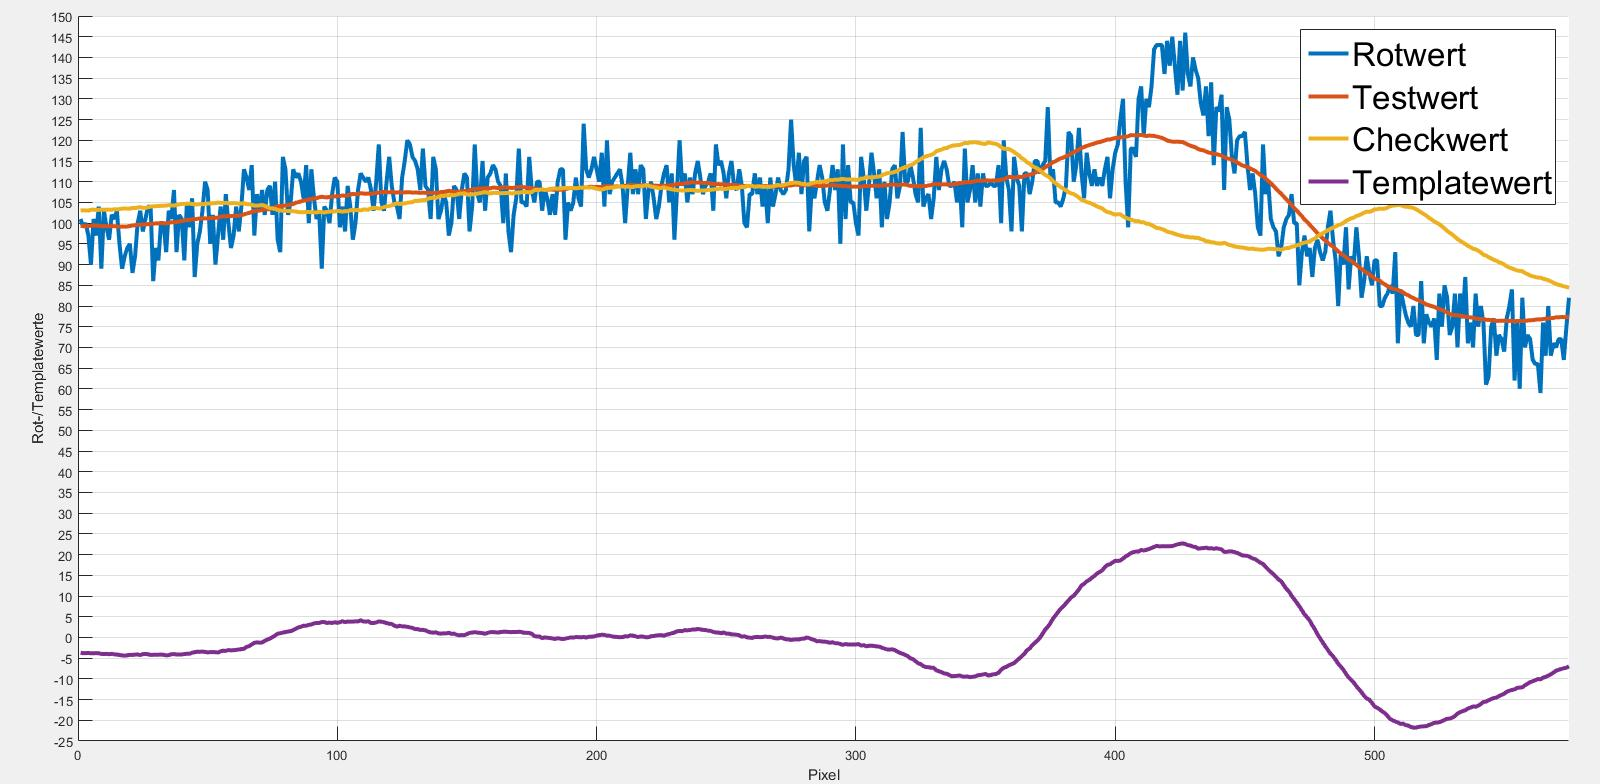
\includegraphics[height=0.33\textheight,width=0.5\textwidth]{1rotRealGut.jpg}\label{redCurve_real}}
\end{tabular}
\caption{Helligkeit und Rotwert im echten Testbild}
\end{figure}

\begin{figure}[H]
\begin{tabular}{cc}
\multicolumn{2}{c}{\subfloat[Originalbild]{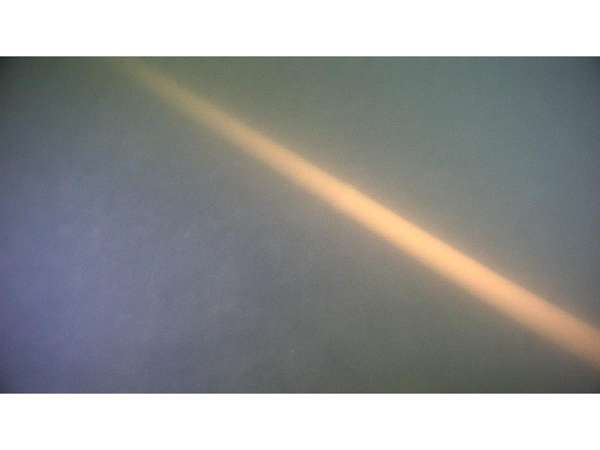
\includegraphics[height=0.33\textheight,width=0.5\textwidth]{imageProcessing/realPipe/004orgImstart.jpg}}}\\
%\subfloat[Originalbild]{\includegraphics[height=0.33\textheight,width=0.5\textwidth]{imageProcessing/3orgImFin.jpg}}\\
\subfloat[Helligkeitsverlauf einer Bildzeile im oberen Drittel des Bildes]{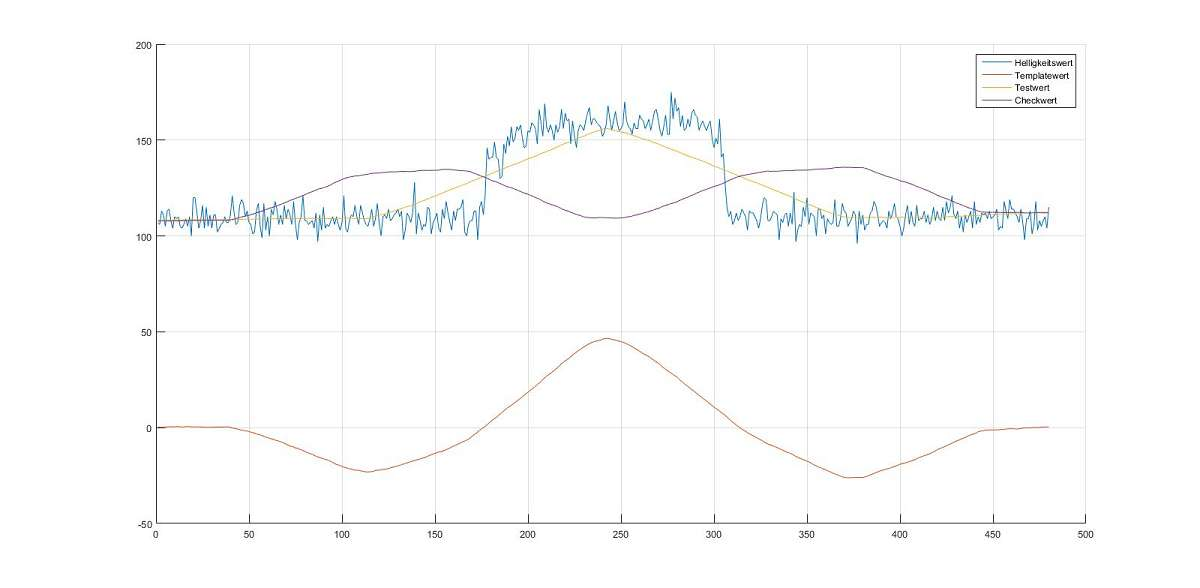
\includegraphics[height=0.33\textheight,width=0.5\textwidth]{hellSimImage.jpg}\label{brightCurve_sim}}&
\subfloat[Rotwertverlauf einer Bildzeile im oberen Drittel des Bildes]{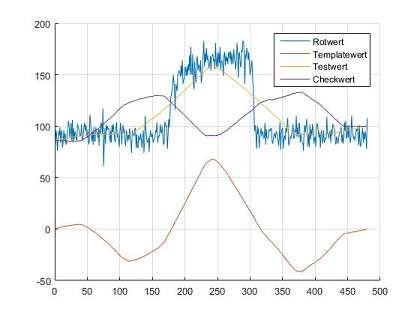
\includegraphics[height=0.33\textheight,width=0.5\textwidth]{rotSimImage.jpg}\label{redCurve_sim}}
\end{tabular}
\caption{Helligkeit und Rotwert im Simulationsbild}
\end{figure}

Im weiteren Verlauf wird auf dem Binärbild gearbeitet. Nach dem Vorbild von Wang et al. \cite{wang2004lane} wird das Bild in drei Segmente unterteilt.\\
In jedem Segment wird dann mithilfe des \rans Algorithmus ein Rechteck gesucht. Da ein \rans standardmäßig Linien erkennt habe ich den Algorithmus insofern umgeschrieben, dass keine Linie zwischen zwei zufälligen Punkten erzeugt wird, sondern ein Rechteck um einen zufälligen Punkt mit einer zufälligen Orientierung. Die Breite dieses Rechtecks wird dabei durch den erwarteten Objektdurchmesser bestimmt. Für jeden Punkt wird dann geprüft, ob er im Rechteck liegt (ein Inlier ist). Gemäß des \rans wird das Rechteck mit den meisten Inliern gewählt.\\
Somit gibt es für jedes Bild bis zu drei Objektposen. Durch das unterteilen in Segmente lässt sich zum Einen bestimmen, in wie vielen Segmenten ein Objekt erkannt wurde (entspricht der \textit{Länge} des Objektes im Bild). Des weiteren kann ein gebogener Verlauf oder ein abgeknicktes Objekt im Bild sinnvoll erkannt werden.\\
In den ersten Tests dieses Verfahrens ist ersichtlich geworden, dass es einen Tradeoff \todo{richtige wortwahl?} zwischen Geschwindigkeit und Erkennungsgüte gab. Die Erkennung wurde besser, je mehr maximale Iterationen dem \rans erlaubt wurden. Da der \rans jedoch auf jedes der drei Segmente separat angewendet wird, wird bei steigender Iterationsanzahl die Geschwindigkeit deutlich reduziert. Für eine zuverlässige Erkennung waren zu viele Iterationen nötig, sodass das Verfahren nicht einsetzbar wäre.\\
Als Lösung für dieses Probleme habe ich die möglichen erzeugten Rechtecke für den \rans begrenzt. Da das Template nur in horizontaler Richtung auf das Bild angewendet wird sind horizontal liegende Objekte im Binärbild nicht sichtbar. Aufgrund dieser Tatsache lassen sich die Rechtecke auf eher vertikale Ausrichtungen beschränken. Durch diese Maßnahme wurden die benötigten Iterationen für ein zuverlässiges Ergebnis drastisch reduziert. Daraus resultiert jedoch die Problematik zu stark horizontale Objekte nicht mehr richtig erkennbar sind [\ref{detecFail}]\\
Der zweite Faktor, der die Geschwindigkeit der Objekterkennung verringerte war die Menge der Punkte im Binärbild. So mussten für jede Iteration des \rans für jeden Punkt geprüft werden, ob der Punkt im Rechteck liegt. In den Testbildern der Simulation lag die Anzahl der Punkte teilweise bei weit über $10000$, was in Kombination mit $200$ Iterationen zu einem unperformanten führte.\\ Zum lösen dieses Problems wurden vorm Einsatz des \rans die Punktanzahl verringert, indem nur jedes dritte Pixel betrachtet wird und diese den Wert aller seiner Nachbarpixel erhält. \todo{Grafik?} Somit konnte die Punktanzahl zuverlässig auf unter $2000$ verringert werden, was zu einer deutlichen Beschleunigung ohne nennenswerte Verschlechterung der Ergebnisse führte.
\begin{figure}[H]
\centering
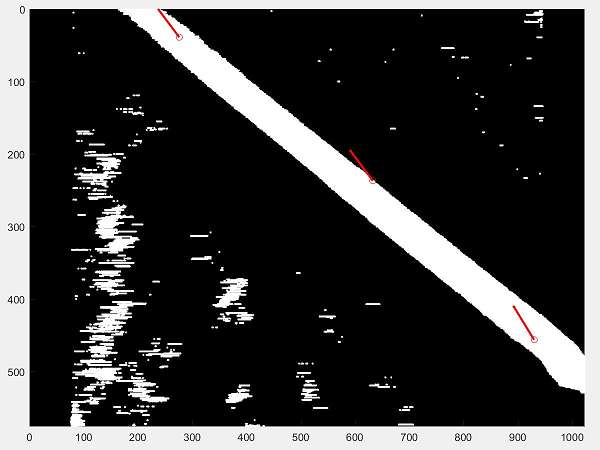
\includegraphics[scale=0.5]{imageProcessing/realPipe/004detectedImage.jpg}
\caption{Falsche Erkennung aufgrund der Beschränkung der Ausrichtungen für den \rans}
\label{detecFail}
\end{figure}
\subsubsection*{Gewicht der erkannten Punkte}
\label{sec_weights}
Im Abschnitt zum Schätzverfahren [\ref{sec_curveFit}] wird die Notwendigkeit einer gewichteten Erkennung erläutert. Hierfür liefert die Objekterkennung wichtige Faktoren zum bestimmen eines Gewichts.\\
\begin{itemize}
\item \textbf{numParts:} Länge des Objektes im Bild. Die erkannten Punkte werden nach Parallelität ihrer Ausrichtung und Nähe zueinander untersucht. Somit wird untersucht in wievielen Segmenten das Objekt fortgeführt wird.
\item \textbf{area:} Um den Punkt wird ein Rechteck gelegt, dass der Breite des Objektes und der Höhe des Segmentes entspricht. \textbf{area} gibt einen relativen Wert an, wie ausgefüllt dieses Rechteck ist.
\item \textbf{peakheight:} Es wird der Mittelwert aller der Helligkeit innerhalb des Rechtecks berechnet und mit dem allgemeinen Helligkeitswert des Bildes verglichen. \textbf{peakheight} dieses Verhältnis relativ an.
\item \textbf{fitsBorder:} Gibt als boolean an, ob das erkannte Objekt der berechneten Objektbreite passt.
\item \textbf{relativeCount:} Gibt das Verhältnis von Punkten im Binärbild, die zum Objekt passen und der Gesamtzahl der Punkte an.
\end{itemize}